\documentclass[12pt]{article}
\usepackage[utf8]{inputenc}
\usepackage{amsmath, amssymb, amsthm}
\usepackage{enumitem}
\usepackage{geometry}
\usepackage{fancyhdr}
\usepackage{pgfplots}
\usepackage{tikz}
\usepackage{float}
\usepackage{graphicx}
\DeclareMathOperator{\Tr}{Tr}
\DeclareMathOperator{\rng}{rng}
\DeclareMathOperator{\norm}{||}
\DeclareMathOperator{\NN}{\mathbb{N}}
\DeclareMathOperator{\ZZ}{\mathbb{Z}}
\DeclareMathOperator{\QQ}{\mathbb{Q}}
\DeclareMathOperator{\RR}{\mathbb{R}}
\DeclareMathOperator{\CC}{\mathbb{C}}

% Page setup
\setlength{\headheight}{15pt}
\geometry{letterpaper, margin=1in}
\setlength{\parindent}{0pt}
\setlength{\parskip}{1em}
\pagestyle{fancy}
\fancyhf{}
\fancyhead[L]{\textbf{Sebastian Griego}}  % Replace with your name
\fancyhead[C]{\textbf{Math Modeling}}  % Replace with your course name
\fancyhead[R]{\textbf{Assignment \#2}}  % Replace with your assignment number
\fancyfoot[C]{\thepage}

\newenvironment{problem}[1]{
    \textbf{Problem #1:}
}{
    \rmfamily \vspace{1em}
}

\newenvironment{solution}{
    \textbf{Solution:}
    
}{
    
    \vspace{2em}
}

\begin{document}

\title{Homework \#2}  % Replace with the homework number
\author{Sebastian Griego}  % Replace with your name

\begin{problem}{4}
    The favorite food of the tiger shark is the sea turtle. A two-species prey-predator model is given by
    \[
        \begin{aligned}
            \frac{dP}{dt} &= P(a - bP - cS)\\
            \frac{dS}{dt} &= S(-k + \lambda P)
        \end{aligned}
    \]
    where \(P\) is the sea turtle, \(S\) is the shark, \(a, b, c, k, \lambda > 0\).
    \begin{enumerate}
        \item Let \(b = 0\) and the value of \(k\) is increased. Ecologically, what is the interpretation of increasing \(k\) and what is its effect on the non-zero equilibrium populations of sea turtles and sharks?
        \item Obtain all the equilibrium solutions for \(b = 0\) and \(b \neq 0\).
        \item Obtain the linearized system of differential equations about the equilibrium point \(P^* = \frac{k}{\lambda}\) and \(S^* = \frac{a}{c} - \frac{bk}{c\lambda} > 0\), which can be put in the form
        \[
            \begin{aligned}
                \frac{dP_1}{dt} &= \frac{k}{\lambda} (-bP_1 - cS_1)\\
                \frac{dS_1}{dt} &= \lambda P_1 \left(\frac{a}{c} - \frac{bk}{c\lambda}\right)
            \end{aligned}
        \]
        \item Obtain the conditions for which the linearized system is stable.
        \item Draw the solution curves in the phase plane with \(a = 0.5, b = 0.5, c = 0.01, k = 0.3, \lambda = 0.01\). What do you expect to happen to the dynamics of the model if \(c=0\)?
    \end{enumerate}
\end{problem}

\begin{solution}
    \begin{enumerate}
        \item Ecological Interpretation and Effect of Increasing \(k\)
        
        When \(b = 0\), the equation for \(\frac{dP}{dt}\) is
        \[
            \frac{dP}{dt} = P(a - cS)
        \]
        Increasing \(k\) in the equation \(\frac{dS}{dt} = S(-k + \lambda P)\) can be interpreted as increasing the  death rate of the shark population or decreasing the reproduction reproduction rate.

        Set the equations equal to zero to find the equilibrium points:
        \[
            \begin{aligned}
                P(a - cS) &= 0 \\
                S(-k + \lambda P) &= 0
            \end{aligned}
        \]
        Solving for non-zero equilibrium points gives
        \[
            P^* = \frac{k}{\lambda}
        \]
        \[
            S^* = \frac{a}{c}
        \]
        As \(k\) increases, \(P^*\) increases, so the equilibrium population of sea turtles increases. \(S^*\) does not depend on \(k\), so the equilibrium population of sharks does not change.

        \item Equilibrium Solutions for \(b = 0\) and \(b \neq 0\)

        For \(b = 0\):
        The system becomes:
        \[
            \begin{aligned}
                \frac{dP}{dt} &= P(a - cS) \\
                \frac{dS}{dt} &= S(-k + \lambda P)
            \end{aligned}
        \]
        The trivial equilibrium points are \(P = 0\) and \(S = 0\). The non-zero equilibrium points are found by solving:
        \[
            \begin{aligned}
                a - cS &= 0 \implies S = \frac{a}{c} \\
                -k + \lambda P &= 0 \implies P = \frac{k}{\lambda}
            \end{aligned}
        \]
        The equilibrium points are:
        \[
            \begin{aligned}
                \left( P_0^*, S_0^* \right) &= (0,0)\\
                \left( P_1^*, S_1^* \right) &= \left( \frac{k}{\lambda}, \frac{a}{c} \right) \\
            \end{aligned}
        \]

        For \(b \neq 0\):
        The equations are:
        \[
            \begin{aligned}
                P(a - bP - cS) &= 0 \\
                S(-k + \lambda P) &= 0
            \end{aligned}
        \]
        The trivial equilibrium points are \(P = 0\) and \(S = 0\). Solving for non-zero equilibria:
        \[
            \begin{aligned}
                a - bP - cS &= 0 \\
                -k + \lambda P &= 0 \implies P = \frac{k}{\lambda}
            \end{aligned}
        \]
        Substitute \(P = \frac{k}{\lambda}\) into the first equation:
        \[
            a - b\left(\frac{k}{\lambda}\right) - cS = 0 \implies S = \frac{a}{c} - \frac{bk}{c\lambda}
        \]
        Therefore, the non-zero equilibrium points are
        \[
            \begin{aligned}
                \left(P^*_0, S^*_0\right) &= \left(0, 0\right)\\
                \left(P^*_1, S^*_1\right) &= \left(\frac{k}{\lambda}, \frac{a}{c} - \frac{bk}{c\lambda}\right)
            \end{aligned}
        \]

        \item Linearization of the System Around the Equilibrium Point \( \left( P^*, S^* \right) \)

        Compute the Jacobian Matrix
        \[
            \begin{aligned}
                J &= \begin{pmatrix}
                    \frac{\partial}{\partial P}\left(\frac{dP}{dt}\right) & \frac{\partial}{\partial S} \left(\frac{dP}{dt}\right) \\
                    \frac{\partial}{\partial P} \left(\frac{dS}{dt}\right) & \frac{\partial}{\partial S} \left(\frac{dS}{dt}\right)
                \end{pmatrix}\\
                &= \begin{pmatrix}
                    a - 2bP - cS & -cP \\
                    \lambda S & -k + \lambda P
                \end{pmatrix}
            \end{aligned}
        \]
        Evaluate the Jacobian at the equilibrium point
        \[
            P^* = \frac{k}{\lambda} \quad S^* = \frac{a}{c} - \frac{bk}{c\lambda}
        \]
        Substitute \( P^* \) and \( S^* \) into the Jacobian matrix:
        \[
            J(P^*, S^*) = \begin{pmatrix}
                a - 2b\left(\frac{k}{\lambda}\right) - c\left(\frac{a}{c} - \frac{bk}{c\lambda}\right) & -c\left(\frac{k}{\lambda}\right) \\
                \lambda\left(\frac{a}{c} - \frac{bk}{c\lambda}\right) & -k + \lambda\left(\frac{k}{\lambda}\right)
            \end{pmatrix}.
        \]
        Simplify the matrix:
        \[
            \begin{aligned}
                J(P^*, S^*) &= \begin{pmatrix}
                    a - \frac{2bk}{\lambda} - \left(a - \frac{bk}{\lambda}\right) & -\frac{ck}{\lambda} \\
                    \frac{\lambda a}{c} - \frac{bk}{c} & 0
                \end{pmatrix}\\
                &= \begin{pmatrix}
                    -\frac{bk}{\lambda} & -\frac{ck}{\lambda} \\
                    \frac{\lambda a}{c} - \frac{bk}{c} & 0
                \end{pmatrix}
            \end{aligned}
        \]
        Write out the matrix form:
        \[
            \begin{pmatrix}
                \frac{dP_1}{dt} \\
                \frac{dS_1}{dt}
            \end{pmatrix}
            =
            \begin{pmatrix}
                -\frac{bk}{\lambda} & -\frac{ck}{\lambda} \\
                \frac{\lambda a}{c} - \frac{bk}{c} & 0
            \end{pmatrix}
            \begin{pmatrix}
                P_1 \\
                S_1
            \end{pmatrix}
        \]
        Write out the system of equations:
        \[
            \begin{aligned}
                \frac{dP_1}{dt} &= -\frac{bk}{\lambda} P_1 - \frac{ck}{\lambda} S_1 \\
                \frac{dS_1}{dt} &= \left( \frac{\lambda a}{c} - \frac{bk}{c} \right) P_1
            \end{aligned}
        \]
        This can also be written as:
        \[
            \begin{aligned}
                \frac{dP_1}{dt} &= \frac{k}{\lambda} (-bP_1 - cS_1)\\
                \frac{dS_1}{dt} &= \lambda P_1 \left(\frac{a}{c} - \frac{bk}{c\lambda}\right)
            \end{aligned}
        \]
        \item Conditions for Stability of the Linearized System
        
        Consider the Jacobian matrix evaluated at the equilibrium point \( \left( P^*, S^* \right) \):
        \[
            J(P^*, S^*) = \begin{pmatrix}
                -\frac{bk}{\lambda} & -\frac{ck}{\lambda} \\
                \frac{\lambda a}{c} - \frac{bk}{c} & 0
            \end{pmatrix}
        \]
        The system is stable when the trace of the Jacobian is negative and the determinant is positive.
        \[
            \begin{aligned}
                \Tr(J) &= -\frac{bk}{\lambda} \\
                \det(J) &= \left(0 - \left(-\frac{ck}{\lambda}\right)\left(\frac{\lambda a}{c} - \frac{bk}{c\lambda}\right)\right) = \frac{ck}{\lambda}\left(\frac{\lambda a}{c} - \frac{bk}{c\lambda}\right) = ak - \frac{bk^2}{c\lambda^2}
            \end{aligned}
        \]
        For stability, we need:
        \[
            \begin{aligned}
                \Tr(J) &< 0 \implies -\frac{bk}{\lambda} < 0\\
                \det(J) &> 0 \implies ak - \frac{bk^2}{c\lambda^2} > 0
            \end{aligned}
        \]

        \item Phase Plane
        
        Parameters:
        \[
            a = 0.5, \quad b = 0.5, \quad c = 0.01, \quad k = 0.3, \quad \lambda = 0.01
        \]
        
        Equilibrium Point:
        \[
            P^* = \frac{k}{\lambda} = \frac{0.3}{0.01} = 30
        \]
        \[
            S^* = \frac{a}{c} - \frac{bk}{c\lambda} = \frac{0.5}{0.01} - \frac{0.5 \cdot 0.3}{0.01 \cdot 0.01} = 50 - 1500 = -1450
        \]
        
        \( S^* \) cannot be negative because there can't be a negative number of sharks so this equilibrium point is not feasible. The only equilibrium point is the trivial equilibrium \( (0, 0) \).
        
        Phase Plane Dynamics:
                
        The Jacobian at \( (0, 0) \) is:
        \[
            J(0, 0) = \begin{pmatrix}
                a & -c \cdot 0 \\
                \lambda \cdot 0 & -k
            \end{pmatrix} = \begin{pmatrix}
                0.5 & 0 \\
                0 & -0.3
            \end{pmatrix}
        \]
        
        The eigenvalues of this matrix are \( \lambda_1 = 0.5 \) and \( \lambda_2 = -0.3 \). Since one eigenvalue is positive and the other is negative, the origin is a saddle.
        
        The phase plan is on the next page.
        
        If \( c = 0 \), the turtle population \( P \) follows logistic growth unaffected by the sharks. The shark population still depends on the turtle population.

        Graphs:
        \begin{figure}[H]
            \centering
            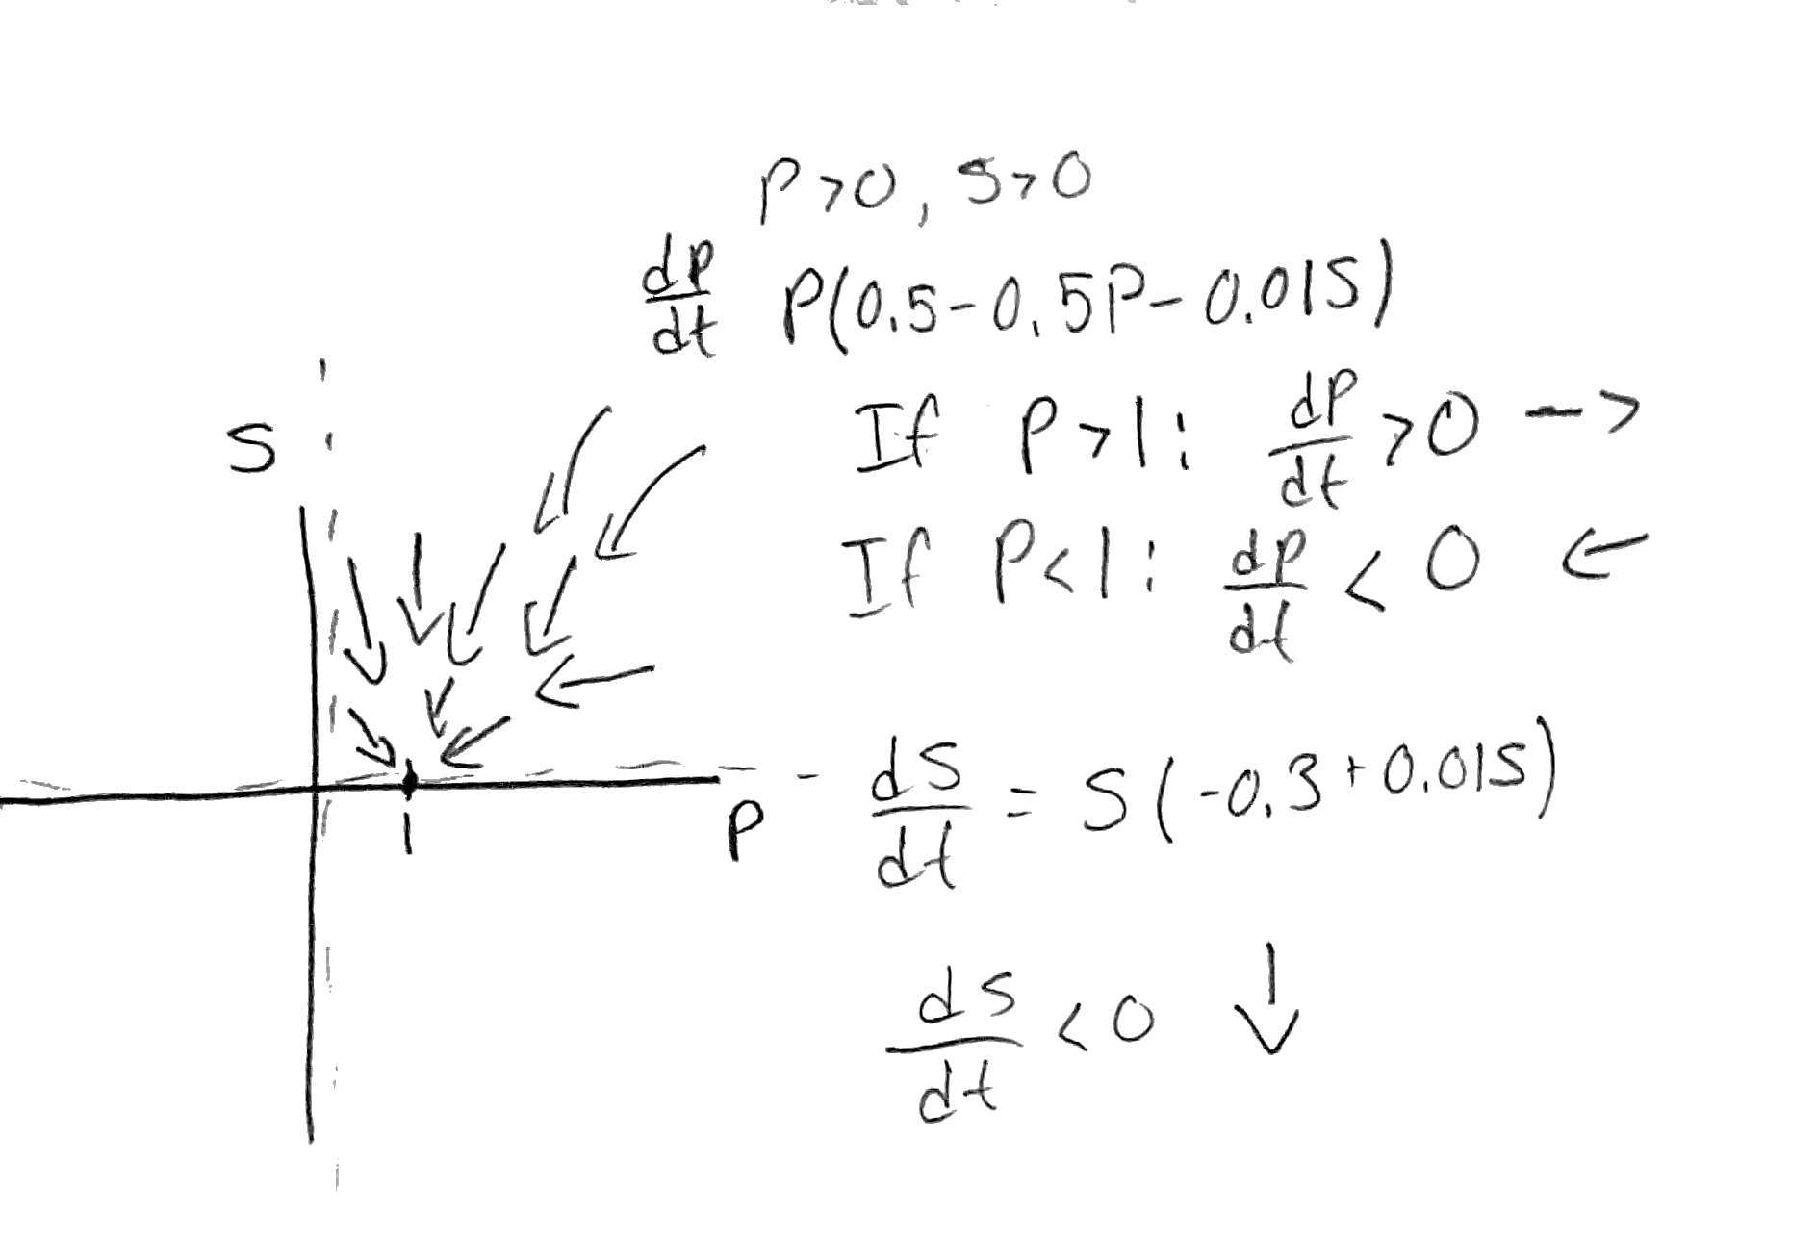
\includegraphics[width=0.8\textwidth]{Graph3.pdf}
        \end{figure}
    \end{enumerate}
\end{solution}

\end{document}